\documentclass[11pt,a4paper]{article}
\pdfoutput=1

\usepackage[T1]{fontenc}
\usepackage[utf8]{inputenc}
\usepackage[margin=1in]{geometry}
\usepackage{amsmath,amssymb,amsthm,mathtools}
\usepackage{bm}
\usepackage{booktabs}
\usepackage{graphicx}
\usepackage{microtype}
\usepackage{xcolor}
\usepackage{url}
\usepackage[colorlinks=true,allcolors=blue!55!black]{hyperref}

\newtheorem{theorem}{Theorem}
\newtheorem{lemma}{Lemma}
\newcommand{\cL}{\mathcal{L}}
\newcommand{\cD}{\mathcal{D}}
\newcommand{\R}{\mathbb{R}}
\newcommand{\C}{\mathbb{C}}
\newcommand{\Tr}{\operatorname{Tr}}
\newcommand{\rank}{\operatorname{rank}}
\newcommand{\dd}{\mathrm{d}}
\newcommand{\ket}[1]{\lvert #1\rangle}
\newcommand{\bra}[1]{\langle #1\rvert}
\newcommand{\dyad}[2]{\lvert #1\rangle\!\langle #2\rvert}
\setcounter{MaxMatrixCols}{12}

\title{Finite-radius rank-two local optimality for a qubit quantum-embeddability ansatz}
\author{Xiaojian Zeng\\
\small PBC School of Finance, Tsinghua University, 100190\\
\small \href{mailto:xiaojianzeng@foxmail.com}{xiaojianzeng@foxmail.com}}
\date{}

\begin{document}

\maketitle

\begin{abstract}
Classical transition matrices obtained by preparing and measuring a qubit in
one fixed basis form a constrained subset when the intervening evolution is a
time-homogeneous quantum dynamical semigroup.  A recent numerical study
proposed that a four-parameter Hamiltonian--one-jump family generates the
boundary of the qubit set.  We do not resolve that global question.  Instead,
we prove a computer-assisted finite-radius result at one stationary point of
the section $a=1/2$.  In an explicit eleven-coordinate, gauge-fixed canonical
chart for Kossakowski rank at most two, an interval-Newton enclosure fixes the
one-jump point and outward-rounded matrix-exponential derivatives bound the
Hessian on the complete cube $|y_i|\leq10^{-4}$.  The smallest directed
Gershgorin lower endpoint is larger than $0.0333886$, which implies
\[
 b(y)-b_\star\geq 0.0165\,\lVert y\rVert_2^2
 \quad\text{whenever}\quad a(y)=1/2.
\]
Here $b_\star=0.02261621659234744314\ldots$.  A 320-bit replay and a separately
constructed complex matrix-unit calculation provide independent diagnostics.
Thus a genuinely transverse second dissipative amplitude cannot improve the
tradeoff inside this normalized neighborhood.  The statement excludes
rank-three generators, distant rank-two charts, global optimization,
unbounded parameter tails, and any identification of the true boundary.
\end{abstract}

\section{Introduction}

The embedding problem asks whether a stochastic transition matrix can arise
from continuous-time memoryless dynamics.  Allowing a finite-dimensional
quantum system between classical preparation and measurement enlarges the
set of possible stochastic matrices and leads to the notion of quantum
embeddability~\cite{Korzekwa2021,Shahbeigi2024}.  For a two-level system,
Shahbeigi \emph{et al.} obtained analytical inclusions and exclusions and
compared a general numerical search with a four-parameter family containing
one rank-one jump operator~\cite{Shahbeigi2024}.  Their agreement at entrywise
tolerance $10^{-4}$ motivated the open question of whether that family
generates the boundary of the closed qubit set.

Numerical agreement does not by itself control local optimizer failure,
unbounded rate and time limits, or additional dissipative directions.  The
full boundary question therefore naturally separates into local and global
parts.  This paper addresses one local part: can a second, genuinely
independent jump lower the survival probability $b$ at fixed $a=1/2$ near a
specific stationary point of the one-jump ansatz?

Our contribution is an explicit finite-amplitude answer within Kossakowski
rank at most two.  We construct a canonical chart that removes jump mixing,
jump phase, and the fixed-basis system rephasing at the rank-one point.  The
second jump enters this chart quadratically, so pointwise first-order tests
cannot settle the question.  We instead enclose the full Hessian of a
penalized support functional throughout a normalized coordinate cube using
Arb ball arithmetic~\cite{Johansson2017}.  Strong convexity on the cube then
gives the stated fixed-section inequality by an integral remainder argument.
The assumptions and the exact scope are collected in Theorem~\ref{thm:main}
within the first two sections.

The result is deliberately not presented as a boundary theorem.  It neither
proves that the base point lies on the true quantum-embeddable boundary nor
that it is the global minimum even within the original four-parameter
family.  Its value is narrower: any rank-two counterexample at $a=1/2$ must
leave the displayed local chart cube.  A bounded literature search through
12 September 2026 located no prior finite-radius statement of this form, but
that non-detection is not a priority guarantee.

\section{Model, observable, and the one-jump point}
\label{sec:model}

\subsection{Time-homogeneous qubit dynamics}

Let $\rho$ be a positive semidefinite $2\times2$ matrix of unit trace.  A
time-independent Markovian evolution has a Gorini--Kossakowski--Sudarshan--
Lindblad generator~\cite{Gorini1976,Lindblad1976}
\begin{equation}
 \cL(\rho)=-i[H,\rho]+\sum_k \cD[A_k](\rho),\qquad
 \cD[A](\rho)=A\rho A^\dagger-\frac12\{A^\dagger A,\rho\}.
 \label{eq:gksl}
\end{equation}
Preparation and measurement use the same fixed basis
$\{\ket{0},\ket{1}\}$.  Absorbing the finite evolution time into the
generator, define
\begin{equation}
 T_{ij}=\bra{i}e^{\cL}(\dyad{j}{j})\ket{i},\qquad
 T(a,b)=\begin{pmatrix}a&1-b\\1-a&b\end{pmatrix}.
 \label{eq:observable}
\end{equation}
Thus $a=T_{00}$ and $b=T_{11}$ are dimensionless survival probabilities.
This convention describes each finite generator.  The closed set $Q_2$ in
Ref.~\cite{Shahbeigi2024} additionally permits limits of sequences whose
times or rates are not uniformly bounded; no such limiting argument is used
below.

Write $\rho=(I+\bm r\cdot\bm\sigma)/2$.  For traceless jumps
$A_k=\bm z_k\cdot\bm\sigma$, with
$\bm z_k=\bm u_k+i\bm v_k$, the affine Bloch equation is
\begin{align}
 \dot{\bm r}&=M\bm r+\bm c,\nonumber\\
 M&=2[\bm h]_{\times}
 +2\sum_k\left(\bm u_k\bm u_k^{\mathsf T}
 +\bm v_k\bm v_k^{\mathsf T}
 -(\lVert\bm u_k\rVert^2+\lVert\bm v_k\rVert^2)I_3\right),
 \label{eq:bloch}\
 \bm c&=4\sum_k\bm u_k\times\bm v_k,
\end{align}
where $H=\bm h\cdot\bm\sigma$.  If
$e^{\widetilde M}=\bigl(\begin{smallmatrix}R&\bm d\\0&1\end{smallmatrix}\bigr)$
for $\widetilde M=\bigl(\begin{smallmatrix}M&\bm c\\0&0\end{smallmatrix}\bigr)$,
then
\begin{equation}
 a=\frac{1+R_{zz}+d_z}{2},\qquad
 b=\frac{1+R_{zz}-d_z}{2}.
 \label{eq:ab-bloch}
\end{equation}
The calculation evaluates this full exponential; there is no small-time or
perturbative truncation.

\subsection{Restricted stationary point}

The family proposed in Appendix A of Ref.~\cite{Shahbeigi2024} is
\begin{align}
 H_4&=\sigma_x,\qquad
 A=\sqrt{\gamma}\,\ket{\psi_o(\alpha)}\!\bra{\psi_i(\beta)},\nonumber\\
 \ket{\psi_o(\alpha)}&=(\cos\alpha,i\sin\alpha)^{\mathsf T},\qquad
 \ket{\psi_i(\beta)}=(\cos\beta,i\sin\beta)^{\mathsf T},
 \label{eq:restricted}
\end{align}
with $\gamma\geq0$ and finite time $t>0$.  At fixed $a=1/2$, let
$p=(t,\gamma,\alpha,\beta)$ and solve the five Karush--Kuhn--Tucker equations
\begin{equation}
 a(p)-\tfrac12=0,\qquad
 \nabla_p\bigl[b(p)-\lambda a(p)\bigr]=0.
 \label{eq:kkt}
\end{equation}
Interval Newton proves that the box of componentwise radius $10^{-3}$ about
\begin{equation}
 \begin{aligned}
 p_0={}&(1.6856350198672431,\;0.8285640995933057,\\
       &\quad 0.3147912138228343,\;-0.4934749196785660),\\
 \lambda_0={}&0.03174580990704283
 \end{aligned}
 \label{eq:p0}
\end{equation}
contains a unique solution $(p_\star,\lambda_\star)$ of
Eq.~\eqref{eq:kkt}.  The much tighter propagated enclosure gives
\begin{align}
 b_\star\in[&0.02261621659234744314244509548210769726387405395479335700973522899,
 \nonumber\\[-2mm]
 &0.02261621659234744314244509548210769726387405395479335700973924048].
 \label{eq:bstar}
\end{align}

To express this point in a canonical traceless-jump gauge, set
$q=\sqrt{t\gamma}$, $d=\alpha-\beta$, and $s=\alpha+\beta$.  Removing the
identity part of the jump together with its Hamiltonian compensation gives
\begin{equation}
 h_x=t-\frac{t\gamma}{8}\sin(2d),\qquad
 \bm z=\left(\frac{iq\sin d}{2},
              \frac{q\sin s}{2},
              \frac{q\cos s}{2}\right).
 \label{eq:restricted-map}
\end{equation}
At the solution, the rounded native coordinates are
\begin{equation}
 \begin{aligned}
 (h_x,h_y,h_z,\Re z_y)&=(1.511235499,0,0,-0.105023456),\\
 (\Re z_z,\Im z_x,\Im z_y)&=(0.581493112,0.427275058,0).
 \end{aligned}
 \label{eq:xstar-rounded}
\end{equation}
All certification uses the interval enclosures, not the rounded numbers in
Eqs.~\eqref{eq:p0} and \eqref{eq:xstar-rounded}.

\section{Canonical rank-two chart and main result}
\label{sec:chart}

Consider
\begin{equation}
 \cL_{\bm h,\bm z,\bm w}(\rho)
 =-i[\bm h\cdot\bm\sigma,\rho]
 +\cD[\bm z\cdot\bm\sigma](\rho)
 +\cD[\bm w\cdot\bm\sigma](\rho).
 \label{eq:twojump}
\end{equation}
We use the native real coordinates
\begin{equation}
 x=(h_x,h_y,h_z,\Re z_y,\Re z_z,\Im z_x,\Im z_y,
       \Re\eta_1,\Re\eta_2,\Im\eta_1,\Im\eta_2)
 \in\R^{11}
 \label{eq:native-x}
\end{equation}
and define
\begin{align}
 \bm z&=(i\Im z_x,\,\Re z_y+i\Im z_y,\,\Re z_z),\nonumber\\
 \bm w&=\left(\eta_1,\eta_2,
 -\frac{\overline z_x\eta_1+\overline z_y\eta_2}{\overline z_z}\right).
 \label{eq:chart}
\end{align}
Consequently $\bm z^\dagger\bm w=0$ identically and
\begin{equation}
 C=\bm z\bm z^\dagger+\bm w\bm w^\dagger\succeq0,
 \qquad \rank C\leq2.
 \label{eq:C}
\end{equation}
The certified cube keeps $\Re z_z>0.5813346$, so the rational coordinate in
Eq.~\eqref{eq:chart} is regular.

This chart is locally complete for canonical Kossakowski matrices of rank at
most two near the simple rank-one base point.  Indeed, spectral amplitudes of
a nearby positive semidefinite $C$ give orthogonal $\bm z$ and $\bm w$.
The leading-jump phase and the only system-basis diagonal rephasing relevant
to the observable fix $\Im z_z=0$ and $\Re z_x=0$ on a transverse slice.
The nonzero $z_z$ then yields Eq.~\eqref{eq:chart}.  Jump mixing has been
removed by orthogonality; the remaining phase of $\bm w$ does not change
$\bm w\bm w^\dagger$.

Let $x_\star$ be Eq.~\eqref{eq:restricted-map} at $p_\star$, padded by
$\eta_1=\eta_2=0$.  Let $B\in\R^{11\times11}$ be the fixed invertible
whitening matrix tabulated in Appendix~\ref{app:B}; its full binary64 decimal
representation is supplied as \texttt{whitening-matrix.csv}.  Set
\begin{equation}
 x(y)=x_\star+By,\qquad
 Y_r=\{y\in\R^{11}: |y_i|\leq r\ \text{for all }i\}.
 \label{eq:whitened-chart}
\end{equation}

\begin{theorem}[Finite-radius rank-two local optimality]
\label{thm:main}
For every $y\in Y_{10^{-4}}$, Eq.~\eqref{eq:whitened-chart} defines a finite
time-independent qubit GKSL generator whose Kossakowski rank is at most two.
If its fixed-basis transition matrix satisfies $a(y)=1/2$, then
\begin{equation}
 b(y)-b_\star\geq0.0165\,\lVert y\rVert_2^2.
 \label{eq:main-bound}
\end{equation}
In particular, $y=0$ is the unique minimizer of $b$ on the exact fixed-$a$
section inside this chart cube.
\end{theorem}

The normalization in Eq.~\eqref{eq:whitened-chart} is part of the theorem.
The radius $10^{-4}$ is not an invariant distance in generator space, and
the theorem does not compare with rank-three or distant rank-two generators.

\section{Computer-assisted proof}
\label{sec:proof}

\subsection{Stationary augmented support functional}

Fix the interval-enclosed multiplier $\lambda_\star$ and define
\begin{equation}
 F(y)=b(y)-\lambda_\star a(y),\qquad
 G(y)=F(y)+\bigl(a(y)-\tfrac12\bigr)^2.
 \label{eq:G}
\end{equation}
The seven derivatives of $F$ on the one-jump gauge slice vanish at the exact
root of Eq.~\eqref{eq:kkt}.  The four derivatives in the $\eta$ coordinates
also vanish: $\cD[\bm w\cdot\bm\sigma]$ is quadratic in $\bm w$ and
$\bm w=0$ at the base point.  Since $a(0)=1/2$, the penalty has zero gradient
there.  Hence
\begin{equation}
 \nabla_yG(0)=0
 \label{eq:stationary}
\end{equation}
exactly; this conclusion does not replace a zero equation by a floating-point
residual.

\subsection{Outward-rounded Hessian enclosure}

The implementation propagates value, first derivative, and second derivative
jets through the rational chart and the affine Bloch generator
Eq.~\eqref{eq:bloch}.  Derivatives of the finite-time channel are evaluated
through full block-matrix exponentials.  At first order this is the Fr\'echet map
\begin{equation}
 D e^M[E]=\int_0^1 e^{(1-s)M}E e^{sM}\,\dd s,
 \label{eq:frechet}
\end{equation}
used in matrix-exponential algorithms~\cite{AlMohy2009}; second derivatives
use the corresponding repeated block construction in the certificate.  There
is no polynomial truncation of $e^M$.  Every scalar and matrix operation is
performed with outward-rounded Arb balls at 256-bit precision.

The fixed matrix $B$ whitens the midpoint of $\nabla_x^2G(x_\star)$.  Direct
interval Gershgorin bounds are then applied to the symmetric interval matrix
$H(y)=\nabla_y^2G(y)$ over the complete cube $Y_{10^{-4}}$.  The eleven
directed row lower endpoints are
\begin{equation}
\begin{split}
(&0.0333886328,\ 0.8484794697,\ 0.8331210866,\ 0.9108255037,\\
 &0.9108255035,\ 0.8116418982,\ 0.9121361431,\ 0.8416532932,\\
 &0.8577484555,\ 0.9548488791,\ 0.9548488791).
\end{split}
\label{eq:margins}
\end{equation}
Thus, throughout the cube,
\begin{equation}
 H(y)\succeq0.033\,I_{11}.
 \label{eq:hessian-bound}
\end{equation}
The radius trials are summarized in Fig.~\ref{fig:radii}.  A negative
Gershgorin endpoint at a larger radius only means that this direct enclosure
test is inconclusive there.

\begin{figure}[tb]
 \centering
 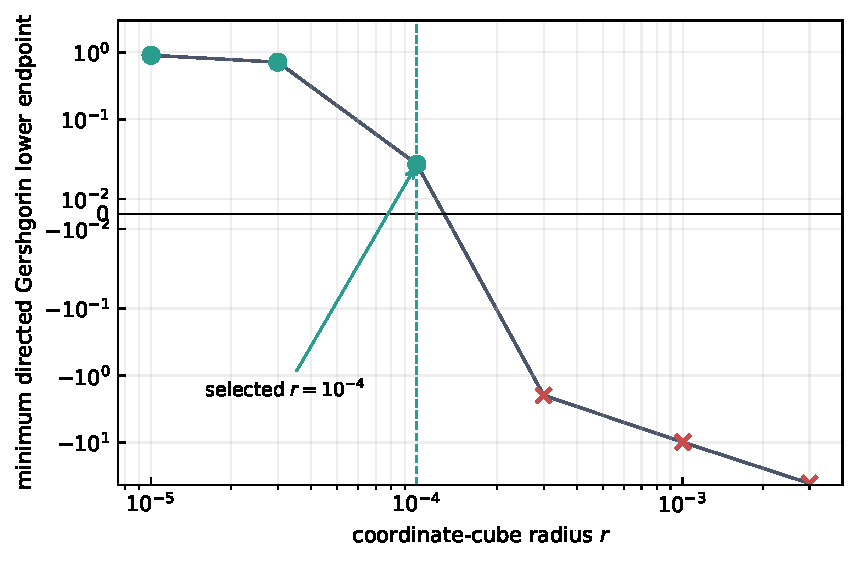
\includegraphics[width=0.92\linewidth]{figures/certificate-radii.pdf}
 \caption{Minimum directed Gershgorin lower endpoint for the interval Hessian
 at each tested coordinate-cube radius.  Filled circles denote a positive
 uniform certificate and crosses denote an inconclusive direct enclosure.
 The largest tested radius passing this criterion is $10^{-4}$.  The plot is
 regenerated directly from the frozen interval JSON record.}
 \label{fig:radii}
\end{figure}

For any $y\in Y_{10^{-4}}$, the segment $sy$ remains inside the cube.  Using
Eqs.~\eqref{eq:stationary} and \eqref{eq:hessian-bound},
\begin{align}
 G(y)-G(0)
 &=\int_0^1(1-s)y^{\mathsf T}H(sy)y\,\dd s\nonumber\\
 &\geq0.0165\,\lVert y\rVert_2^2.
 \label{eq:integral-bound}
\end{align}
On the exact section $a(y)=a(0)=1/2$, both penalty terms vanish and the
support terms cancel, so $G(y)-G(0)=b(y)-b_\star$.  This proves
Theorem~\ref{thm:main}.

\subsection{Error controls and independent diagnostics}

Three additional checks probe distinct failure modes.

First, repeating the complete interval calculation at 320 bits selects the
same radius and preserves every positive row bound.  Precision agreement is
not used as a substitute for outward rounding; both runs are recorded as ball
calculations.

Second, a separate Taylor estimate bounds the Frobenius norm of the full
third-derivative tensor of $G$ by
$3.291\times10^{14}$ on the containing cube.  Combined with a point-Hessian
lower bound greater than $0.9999999999999958$ in whitened coordinates, it
certifies the much smaller radius $9.11\times10^{-15}$.  This deliberately
coarse estimate is an independent analytic remainder check; the
$10^{-4}$ theorem instead uses the stronger uniform-Hessian enclosure.

Third, an implementation constructed directly from the action of
Eq.~\eqref{eq:gksl} on column-major matrix units, rather than from the Bloch
generator, finite-differences the whitened Hessian and corrects random
directions back to $a=1/2$.  It finds
\begin{align}
 \max_{ij}|H^{\mathrm{MU}}_{ij}-\delta_{ij}|&=6.60\times10^{-6},\nonumber\\
 \lambda_{\min}(H^{\mathrm{MU}})&=0.9999998712,\nonumber\\
 \max|\bm z^\dagger\bm w|&=8.56\times10^{-22},\nonumber\\
 \max|a-1/2|&=5.56\times10^{-16}.
 \label{eq:independent-checks}
\end{align}
All sixteen corrected fixed-$a$ trials lie above $b_\star$, with minimum
$b-b_\star=7.996\times10^{-10}$.  These are diagnostic floating-point tests,
not ingredients of the interval proof.

Before the new calculation, two separately derived representations also
reproduced the source model.  At
$(\alpha,\beta,\gamma,t)=(0.2,1.0,0.7,0.9)$, the matrix-unit and affine-Bloch
implementations agree in $(a,b)$ within $4.45\times10^{-16}$.  For
$\gamma=0$, both recover $a=b=\cos^2t$, including the swap at $t=\pi/2$, to
$2.23\times10^{-16}$.  This guards the convention map in
Eq.~\eqref{eq:ab-bloch}; it does not establish global optimization.

\section{Physical meaning and limitations}
\label{sec:limits}

At a rank-one Kossakowski point, a second jump amplitude changes the generator
only at quadratic order.  The chart in Eq.~\eqref{eq:chart} removes the part
that merely remixes the existing jump and retains a genuinely transverse
dissipative amplitude.  Theorem~\ref{thm:main} therefore says that, throughout
the stated normalized neighborhood, opening such a second channel cannot
decrease the fixed-basis survival probability $b$ while preserving
$a=1/2$.  At the edge $\lVert y\rVert_2=10^{-4}$, the certified lower increase
is $1.65\times10^{-10}$; the small numerical scale reflects the local radius,
not a perturbative approximation.

The following exclusions are essential.
\begin{itemize}
 \item The proof treats only the interval-enclosed KKT point at $a=1/2$ and
 the explicit chart $Y_{10^{-4}}$.
 \item Kossakowski rank three is absent.  A rank-three direction is not a
 limit covered by the rank-two chart argument.
 \item No distant rank-two chart, global minimum of the four-parameter
 family, or unbounded time/rate tail is controlled.
 \item The result does not prove that $(1/2,b_\star)$ lies on the boundary of
 $Q_2$, nor does it identify any component of that boundary.
 \item The GKSL equation is an assumed effective model for one qubit.  No
 ancilla, switching, time-dependent control, postselection, or microscopic
 bath statement is included.
\end{itemize}
Consequently the original boundary-generation question remains unresolved.
The present theorem narrows a local counterexample search; it is not a proof
of the one-jump boundary conjecture.

\section{Reproducibility and data availability}

The accompanying source bundle contains the 256-bit interval program, its
KKT and full-slice dependencies, the 320-bit replay, the independent
matrix-unit verifier, machine-readable JSON outputs, the exact whitening
matrix, and regeneration instructions in \texttt{REPRODUCIBILITY.md}.  The
primary certificate uses python-flint 0.9.0/Arb at 256 bits.  The distributed
figure is generated by \texttt{make\_figure.py} from the primary JSON record.
No downloaded third-party paper or upstream code is redistributed in the
submission bundle; the source article and software are identified by their
published references.  Public archival location and licensing of the
project-generated code remain decisions for the author before submission.

\section*{Author contributions and AI-use disclosure}

Xiaojian Zeng supplied the research direction and is the prospective author
of this draft.  Generative-AI systems operating through OpenAI Codex assisted
with literature search, formulation of the local claim, derivations,
production and execution of calculation code, independent computational
checks, figure production, and manuscript drafting.  The prospective author
has not yet confirmed the scientific argument, code, citations, affiliation,
or submission decision and must review the complete work and accept full
responsibility before any submission.

\section*{Competing interests}

No competing-interest statement has yet been confirmed by the prospective
author.

\appendix
\section{Whitening matrix}
\label{app:B}

The rows of $B$ follow the native-coordinate order in
Eq.~\eqref{eq:native-x}; columns multiply $(y_1,\ldots,y_{11})$.  For
readability the display rounds entries smaller than $10^{-12}$ to zero and
the others to six significant digits.  The theorem and interval calculation
use the full binary64 values reproduced in
\texttt{whitening-matrix.csv} and in the primary JSON record.
\begin{equation*}
\resizebox{\linewidth}{!}{$
B\simeq\begin{pmatrix}
0&0&-0.636222&0&0&0.499244&0&0.541959&-0.0692943&0&0\\
-14.4300&0.119842&0&0&0&0&-0.202815&0&0&0&0\\
-1.00410&1.78863&0&0&0&0&0.428288&0&0&0&0\\
0&0&-1.25078&0&0&-0.468106&0&-0.0984261&0.0784189&0&0\\
0&0&-0.427975&0&0&0.650154&0&-0.500656&0.00594322&0&0\\
0&0&0.0933032&0&0&0.111285&0&0.0796181&0.606001&0&0\\
-3.44464&-1.02341&0&0&0&0&0.724775&0&0&0&0\\
0&0&0&0.106061&-0.0597173&0&0&0&0&0.529804&0.202300\\
0&0&0&-0.609665&-1.08279&0&0&0&0&-0.0198155&0.0518949\\
0&0&0&0.0597173&0.106061&0&0&0&0&-0.202300&0.529804\\
0&0&0&1.08279&-0.609665&0&0&0&0&-0.0518949&-0.0198155
\end{pmatrix}$}
\end{equation*}

\bibliographystyle{unsrt}
\bibliography{references}

\end{document}
